\documentclass[areasetadvanced]{scrartcl}

\usepackage[utf8]{inputenc}
\usepackage[T2A]{fontenc}
\usepackage[english,russian]{babel}
\usepackage[footskip=1cm,left=25mm, right=15mm, top=20mm, bottom=20mm]{geometry}
\usepackage{setspace}
\usepackage{amsmath, amssymb}  
\usepackage{graphicx}
\usepackage[final]{pdfpages}
\usepackage{ragged2e}
\usepackage{tikz}
\usetikzlibrary{arrows.meta}
\usepackage{float}
\usepackage{dashrule}
\usepackage{lipsum}
\pagestyle{plain} 
\usepackage{fancyhdr} 
\usepackage{hyperref} 
\usepackage{parskip}
\usepackage{textcomp, enumitem}
\usepackage{indentfirst}
\usepackage{graphicx}
\usepackage{pdflscape}
\usepackage{algorithm}
\usepackage{algpseudocode}
\usepackage{array}  
\usepackage{geometry}
\usepackage{afterpage}
\usepackage{minted}
\setcounter{secnumdepth}{3}  
\setcounter{tocdepth}{3}     
\usepackage{listings} 
\setlength{\parindent}{1.25cm}
\tikzstyle{block} = [rectangle, rounded corners, minimum width=3cm, minimum height=1cm, text centered, draw=black, fill=lightgray]

\setkomafont{sectioning}{\normalfont\bfseries}
\setkomafont{section}{\normalfont\Large\bfseries}
\setkomafont{subsection}{\normalfont\large\bfseries}
\setkomafont{subsubsection}{\normalfont\large\bfseries}
\setkomafont{paragraph}{\normalfont\large\bfseries}

\lstset{
  language=Haskell,
  basicstyle=\ttfamily\small,
  keywordstyle=\color{blue}\bfseries,
  stringstyle=\color{red},
  commentstyle=\color{green!70!black},
  numbers=left,
  numberstyle=\tiny,
  stepnumber=1,
  numbersep=10pt,
  showstringspaces=false,
  breaklines=true,
  frame=single
}

\begin{document}
\thispagestyle{empty}
\newpage
\tableofcontents
\newpage
\section{Описания}
\subsection{Телеграм-бот}
\begin{itemize}
  \item Компонент: интерфейс для взаимодействия с пользователем через Telegram. 
  \begin{itemize}
    \item Передача команд и запросов от пользователя на сервер.
    \item Отображает ответы сервера в чате бота.
  \end{itemize}
\end{itemize}

\subsection{User}
\begin{itemize}
  \item Роль: 
  \begin{itemize}
    \item Telegram пользователь.
  \end{itemize}
  \item Функции: 
  \begin{itemize}
    \item Инициализирует запросы через Telegram бота, такие как: запланировать поездку, добавить заметку к путевой точке и другие.
    \item Делится геолокацией.
    \item Получает сообщения от Telegram бота.
    \item Имеет доступ к эндпоинту /healthcheck без авторизации.
  \end{itemize}
\end{itemize}

\subsection{Admin}
\begin{itemize}
  \item Роли: 
  \begin{itemize}
    \item администратор системы.
  \end{itemize}
  \item Функции: 
  \begin{itemize}
    \item Имеет доступ к эндпоинту /users с авторизацией по API ключу.
    \item Имеет доступ к эндпоинту /healthcheck без авторизации.
  \end{itemize}
\end{itemize}

\subsection{MessageParser}
\begin{itemize}
  \item Компонент: 
  \begin{itemize}
    \item обработка сообщений от Telegram бота.
  \end{itemize} 
  \item Функции: 
  \begin{itemize}
    \item Обрабатывает сообщения от Telegram бота.
    \item Направляет команды в соответствующий модуль.
  \end{itemize}
\end{itemize}

\subsection{TripHelperWorker}
\begin{itemize}
  \item Компонент: 
  \begin{itemize}
    \item модуль помощник c поездкой.
  \end{itemize} 
  \item Функции: 
  \begin{itemize}
  \item Фоново следит за состоянием поездок пользователей.
  \item Уведомляет пользователей об их ближайшей поездке неделю до её
    начала и один день до её начала.
  \item Автоматически делает запланированную поездку текущей при
    наступлений даты её начала.
  \item Автоматически перемещает текущую поездку в историю поездок при
    истечению даты её конца.
  \item Заращивает у пользователя геолокацию в ходе поездки.
  \item Автоматически отмечает путевую точку посещенной, если геолокация
    пользователя входит в определённый радиус вокруг неё.
  \end{itemize}
\end{itemize}
\newpage

\section{Схемы}

\subsection{Сервер}
Основной компонент.
\begin{itemize}
  \item Функции:
  \begin{itemize}
    \item Обрабатывает все веб запросы и запросы от телеграмм бота.
    \item Обеспечение взаимодействия между всеми компонентами.
  \end{itemize}
\end{itemize}

\begin{figure}[H]
  \centering
  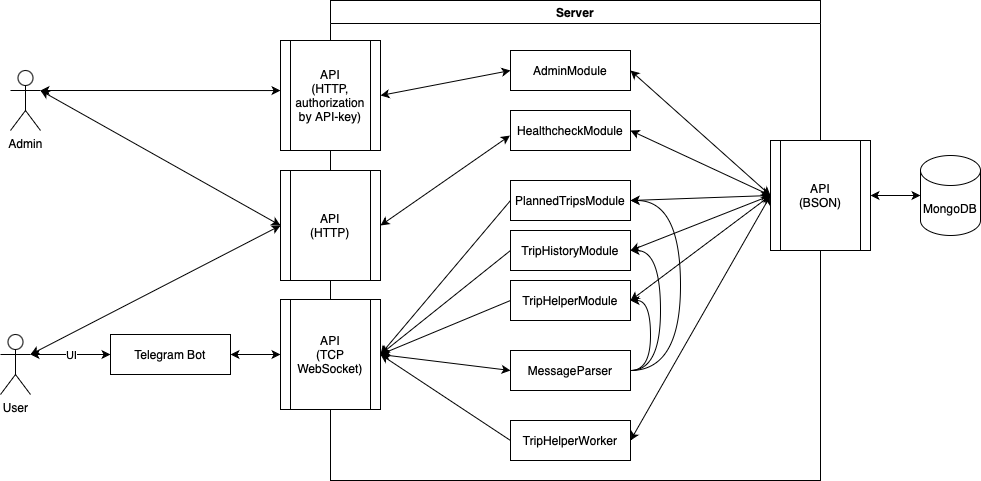
\includegraphics[width=0.7\textwidth]{Server.drawio.png}
  \caption{Схема сервера}
  \label{fig:syntdiag}
\end{figure}
\newpage

\subsection{MongoDB}
\begin{itemize}
  \item База данных: 
  \begin{itemize}
    \item документоориентированная база данных.
  \end{itemize}
  \item Функции: 
  \begin{itemize}
    \item Хранит информацию о администраторах.
    \item Хранит информацию о пользователях и их поездках.
  \end{itemize}
\end{itemize}

\begin{figure}[H]
  \centering
  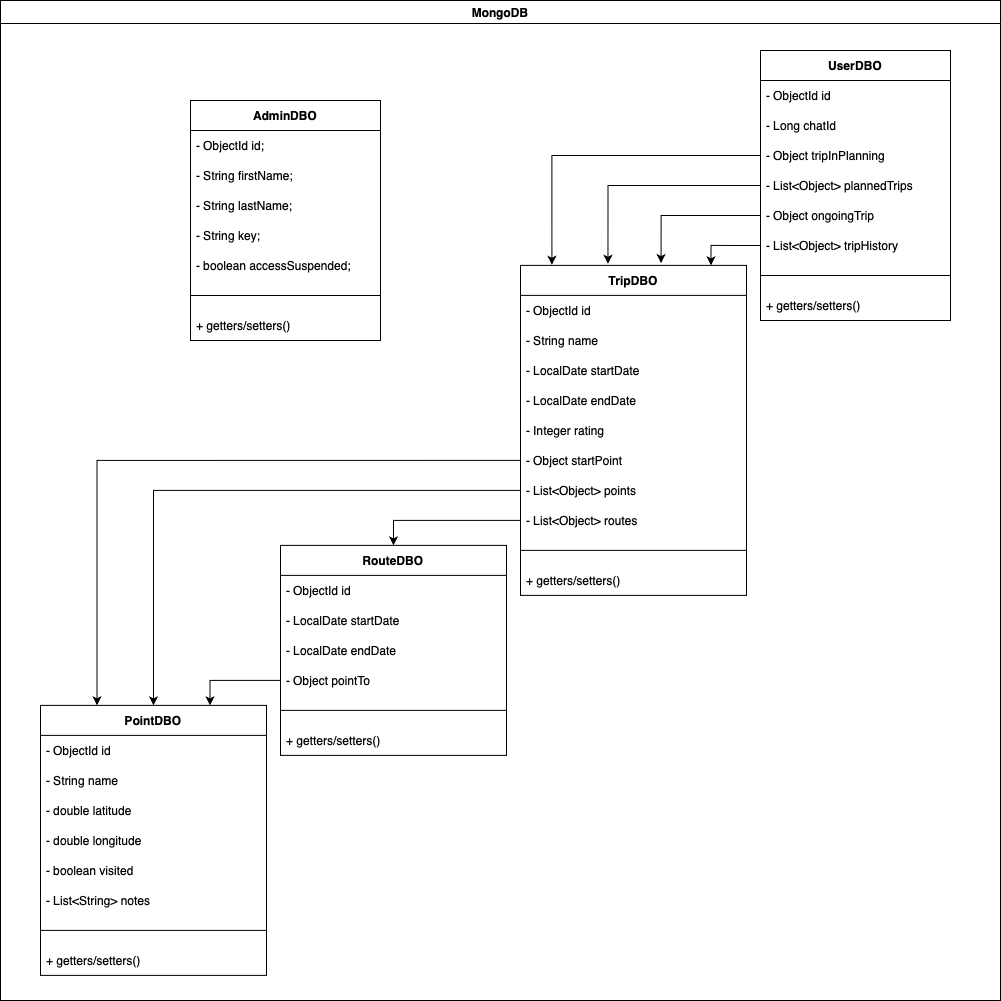
\includegraphics[width=0.7\textwidth]{NewMongoDB.drawio.png}
  \caption{Схема MongoDB (NoSQL)}
  \label{fig:syntdiag}
\end{figure}
\newpage

\subsection{HealthCheckModule}
\begin{itemize}
  \item Компонент: 
  \begin{itemize}
    \item модуль проверки состояния сервера.
  \end{itemize} 
  \item Функции: 
  \begin{itemize}
    \item Реализует эндпоинт /healthcheck для проверки работоспособности сервера и получения списка авторов.
    \item Доступен без авторизации.
  \end{itemize}
\end{itemize}

\begin{figure}[H]
  \centering
  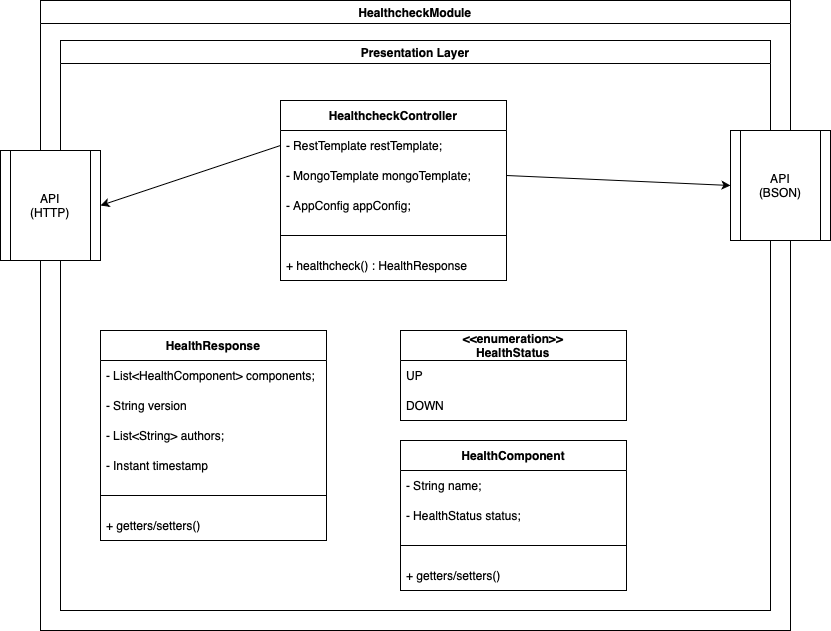
\includegraphics[width=0.7\textwidth]{HealthChecker.drawio.png}
  \caption{Схема HealthChecker}
  \label{fig:syntdiag}
\end{figure}
\newpage

\subsection{AdminModule}
\begin{itemize}
  \item Компонент: 
  \begin{itemize}
    \item модуль администрации системы.
  \end{itemize} 
  \item Функции: 
  \begin{itemize}
    \item Реализует эндпоинт /users, отображающий данные о всех пользователях.
    \item Доступен администраторам с авторизацией.
  \end{itemize}
\end{itemize}

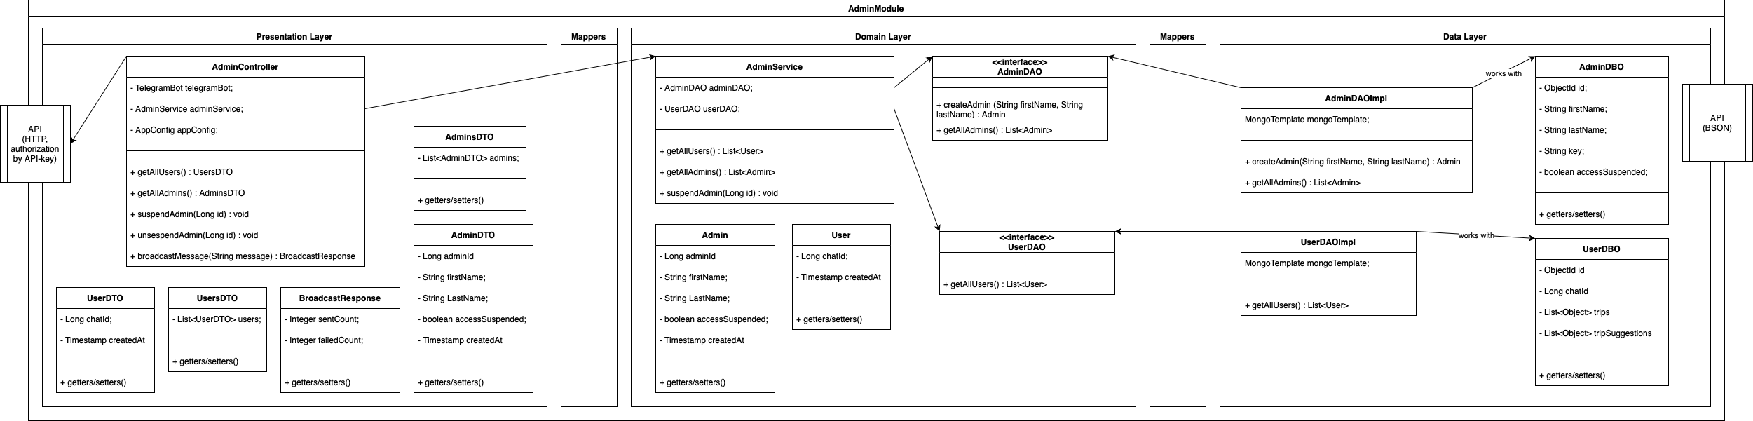
\includepdf[fitpaper]{AdminModule.drawio.pdf}
\newpage

\subsection{PlannedTripsModule}
\begin{itemize}
  \item Компонент: 
  \begin{itemize}
    \item модуль планирования поездок.
  \end{itemize} 
  \item Функции: 
  \begin{itemize}
    \item Обрабатывает команду /showplanned, получение списка запланированных поездок.
    \item Обрабатывает команду /plantrip, запланирование новой поездки.
    \item Обрабатывает команду /addpoint, добавление путевой точки в поездку.
    \item Обрабатывает команду /setstartpoint, установление начальной путевой точки в поездке.
    \item Обрабатывает команду /addroute, добавление маршрута между точками.
    \item Обрабатывает команду /finishplanning, запланирование поездки.
    \item Обрабатывает команду /cancelplanning, отмета планирования.
    \item Обрабатывает команду /deleteplanned, удаление запланированной поездки.
  \end{itemize}
\end{itemize}

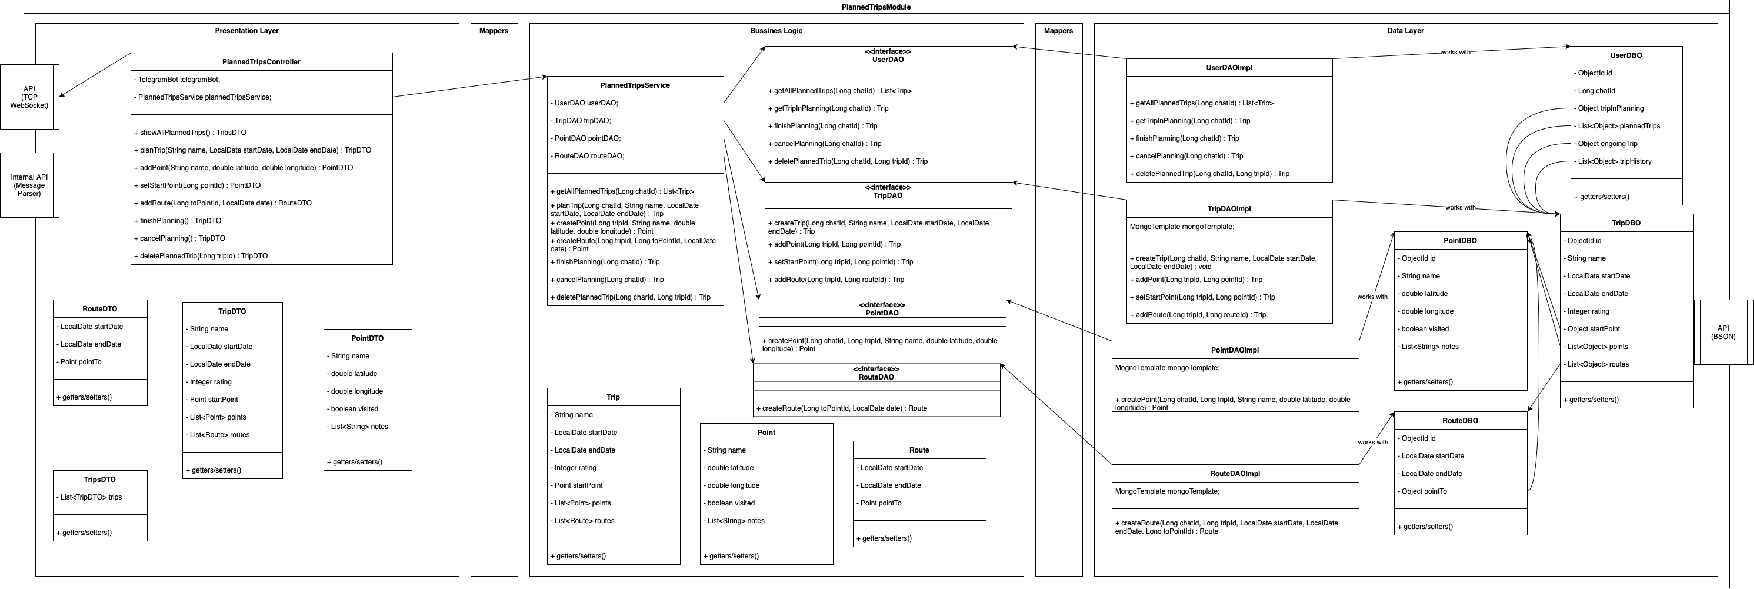
\includepdf[fitpaper]{NewPlannedTripsModule.drawio.pdf}
\newpage

\subsection{TripHelperModule}
\begin{itemize}
  \item Компонент: 
  \begin{itemize}
    \item модуль помощник c поездкой.
  \end{itemize} 
  \item Функции: 
  \begin{itemize}
    \item Обрабатывает команду /showongoingtrip, отображение информации о текущей поездке.
    \item Обрабатывает команду /addnote, добавление заметки к путевой точке одной из поездкой.
    \item Обрабатывает команду /markpoint, мануальная отметка путевой точки текущей поездки как посещенной.
  \end{itemize}
\end{itemize}

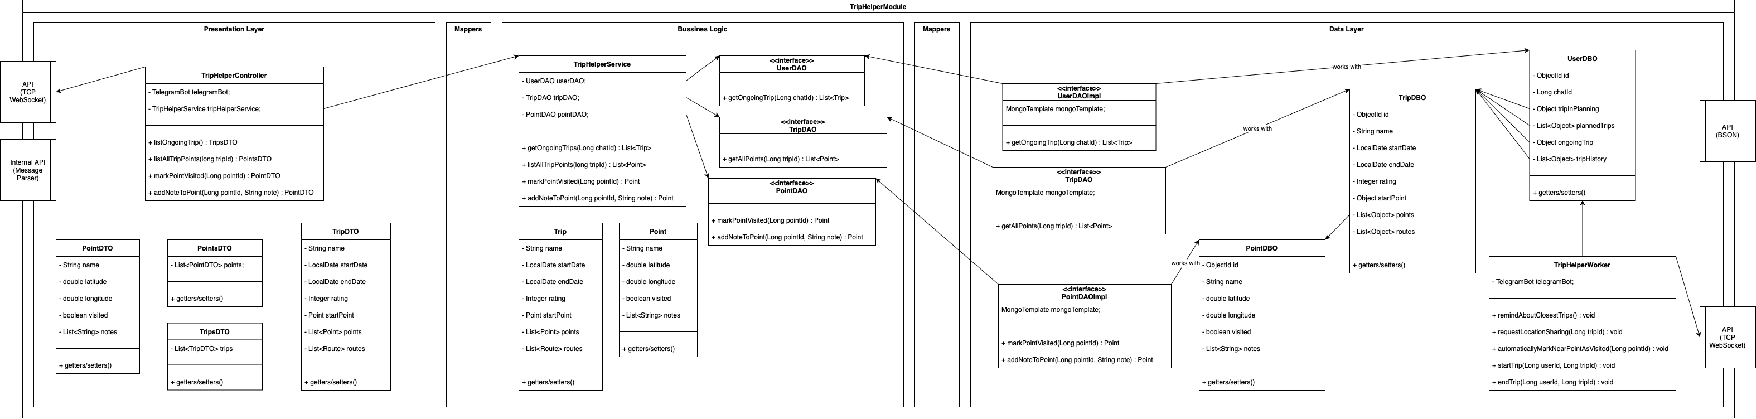
\includepdf[fitpaper]{NewHelperModule.drawio.pdf}
\newpage

\subsection{TripHistoryModule}
\begin{itemize}
  \item Компонент: 
  \begin{itemize}
    \item модуль истории поездок.
  \end{itemize} 
  \item Функции: 
  \begin{itemize}
    \item Обрабатывает команду /triphistory, отображает список всех
    завершенных поездок.
    \item Обрабатывает команду /finisheddetails, отображает подробную
      информацию о конкретной завершенной поездке.
    \item Обрабатывает команду /ratefinished, установливает оценку
      завершенной поездке.
  \end{itemize}
\end{itemize}

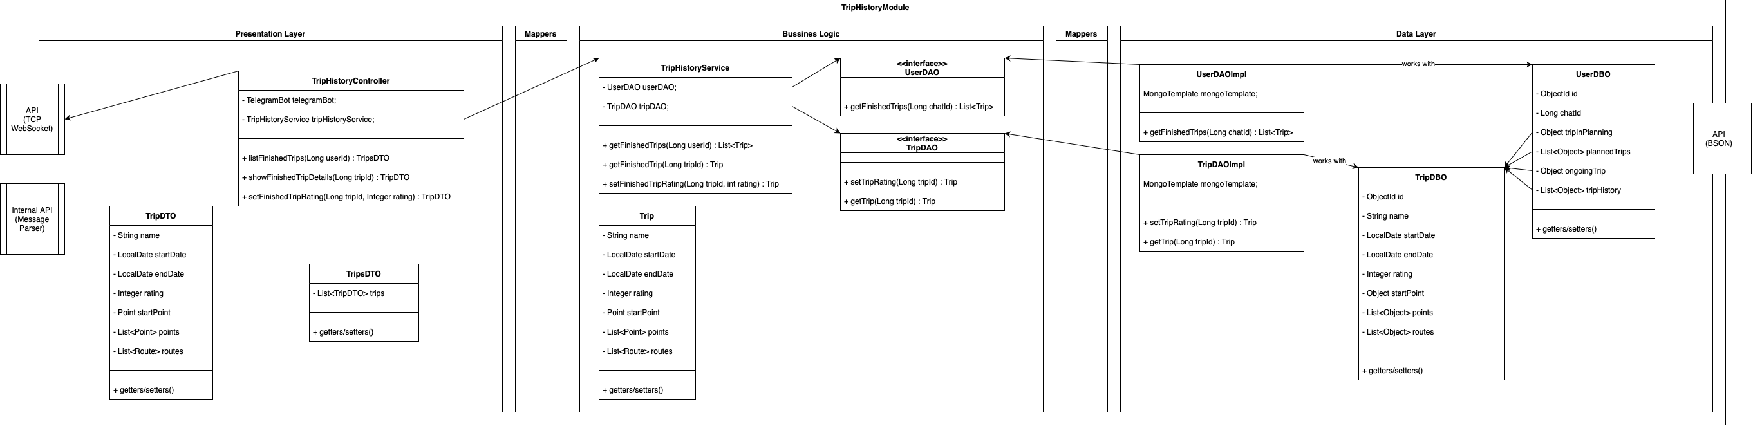
\includepdf[fitpaper]{NewHistoryModule.drawio.pdf}
\newpage


\section{Описание развертывания приложения}

\subsection{Подготовка окружения}
\begin{itemize}
    \item Установка Docker и Docker Compose на сервер.
    \item Настройка переменных окружения (`.env`) для подключения к Telegram API, MongoDB и Kafka.
\end{itemize}

\subsection{Конфигурация инфраструктуры}
\begin{itemize}
    \item Запуск MongoDB и Kafka через Docker Compose.
    \item Настройка репликации и шардинга для MongoDB (если требуется).
    \item Проверка доступности брокера сообщений Kafka.
\end{itemize}

\subsection{Развертывание бота}
\begin{itemize}
    \item Сборка Docker-образа приложения (`docker build`).
    \item Публикация образа в Docker Hub.
    \item Запуск контейнера с ботом на сервере (`docker-compose up`).
\end{itemize}

\section{Сборка приложения}

\subsection{Установка зависимостей}
\begin{itemize}
    \item Запуск `gradle build` для загрузки зависимостей (Spring Boot, Telegram API, MongoDB Driver и т.д.).
    \item Проверка совместимости версий Java (SE 23) и Spring (6.2).
\end{itemize}

\subsection{Сборка Fat JAR}
\begin{itemize}
    \item Генерация исполняемого JAR-файла с помощью Gradle (`./gradlew bootJar`).
    \item Проверка наличия всех зависимостей в `build/libs/`.
\end{itemize}

\subsection{Тестирование}
\begin{itemize}
    \item Запуск unit-тестов (`./gradlew test`).
    \item Проверка покрытия кода (минимум 60\%).
\end{itemize}

\subsection{Создание Docker-образа}
\begin{itemize}
    \item Написание `Dockerfile` с базой на `openjdk:23`.
    \item Копирование JAR-файла и запуск приложения в контейнере.
\end{itemize}

\section{Деплой приложения}

\subsection{Загрузка образа в Docker Hub}
\begin{itemize}
    \item Авторизация (`docker login`).
    \item Пуш образа (`docker push username/trip-planner-bot:latest`).
\end{itemize}

\subsection{Развертывание на сервере}
\begin{itemize}
    \item Запуск MongoDB и Kafka через `docker-compose.yml`.
    \item Развертывание бота в отдельном контейнере.
\end{itemize}

\subsection{Проверка работоспособности}
\begin{itemize}
    \item Тестирование команд бота через Telegram.
    \item Мониторинг логов на предмет ошибок (`docker logs <container\_id>`).
\end{itemize}

\section{Запуск приложения}

\subsection{Локальный запуск (для разработки)}
\begin{itemize}
    \item Запуск MongoDB и Kafka через Docker Compose.
    \item Запуск бота через `./gradlew bootRun`.
\end{itemize}

\subsection{Продуктивный режим}
\begin{itemize}
    \item Запуск всех сервисов через `docker-compose up -d`.
    \item Настройка авто-рестарта при падении (`restart: always`).
\end{itemize}

\subsection{Команды для управления}
\begin{itemize}
    \item Остановка: `docker-compose down`.
    \item Обновление: `docker-compose pull \&\& docker-compose up -d`.
\end{itemize}

\end{document}
